\documentclass[a4paper,11pt]{article}
\usepackage{amsmath,amssymb}
\usepackage[a4paper,left=19mm,right=19mm,top=40mm,bottom=40mm]{geometry}
\usepackage{txfonts}
\usepackage{kotex}
\usepackage{graphicx}
\usepackage{algorithm}
\usepackage{algpseudocode}
\usepackage{fancyvrb}

\begin{document}
\title{자료구조 HW8}
\author{B935394 컴퓨터공학과 장준희}
\maketitle
\newpage
\section{이진 탐색 트리}
\  \ 트리의 구현이나 구조는 저번 과제와 타입을 제외하고는 크게 다르지 않기 때문에, 그다지 어려울 것이 없었다. (스레드 이진 트리로 구현했다.) 다만 예상 출력을 보고 insert를 조금 다르게 수정해야하는 점(이전에는 중복일 경우 넣으면 안됐지만, 이번에는 덮어쓰기하는 점) 그리고 hw8.cpp파일을 보고 함수들을 적당히 수정할 필요가 있었다.Max,Min,Delete같은 경우 우선 hw8.cpp에서 호출만 하므로, 출력이 필요하다면 함수내에서 출력하고, 함수의 반환값 자체는 void가 되는 것이 타당하다고 생각했다. 또, 재귀적방법을 쓸 생각이 없었기 때문에 굳이 노드를 인자로 받을 필요가 없다고 생각했다. 그러나 delete의 경우에는 인자에서 지워버리면 public영역에 있는 함수랑 틀이 같아져 hw8.cpp에서 함수를 불러오지 못했다. private영역의 delete를 지워도 됐겠지만, 노드 인자를 받도록 하였다.

Max나 Min 함수의 경우는 매우 간단했다. 나는 이전 과제에서도 따로 헤더노드를 만들지 않고 대신 최우,좌측 노드의 우,좌자식노드를 0으로 설정해뒀기 때문에, root가 가리키는 노드에서 0이 나올때까지 쭉 왼쪽이나 오른쪽으로만 가면 됐다. Delete의 경우 이전 과제에서는 없는 함수이기 때문에 새로 고민을 했어야했는데, 책에 나온대로 자식이 없을 경우/하나일 경우/둘인 경우로 나눠서 생각을 했다. 아래의 그림은 delete와 주어진 트리의 구조를 보여준다. (파란색 hzhz:~ 는 테스트할 것이 있어 나중에 추가된 것이므로 무시하고 검정색의 노드와 회색의 스레드, NULL을 보면 된다.)\\
\begin{figure}[h]
\begin{center}
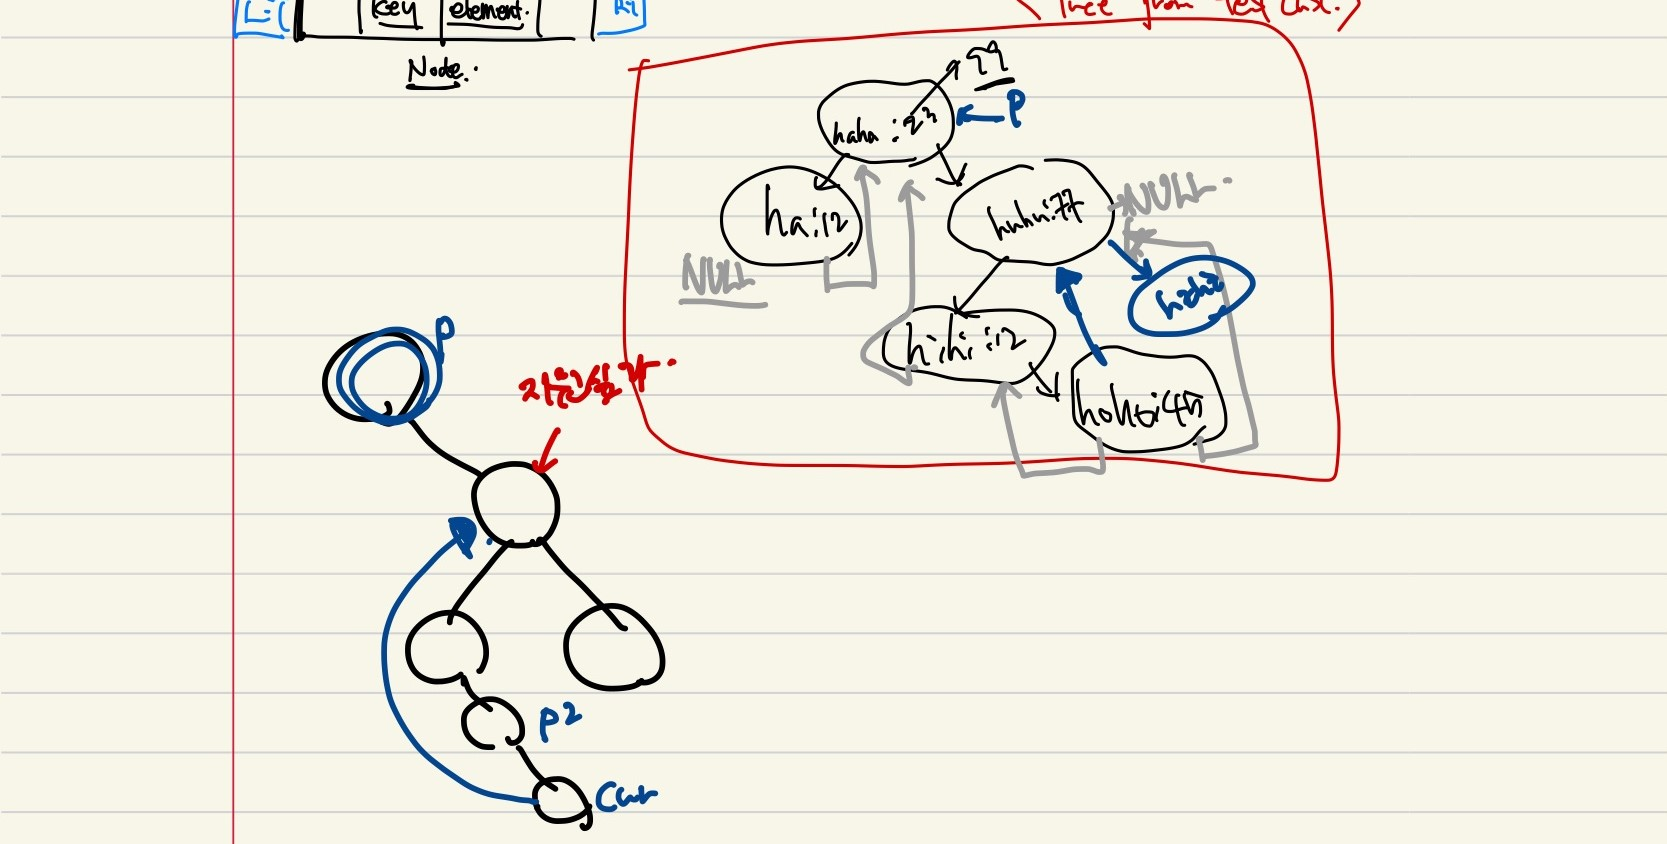
\includegraphics[width=0.6\textwidth]{bst}
\caption{스레드이진탐색트리}
\label{fig:fig1}
\end{center}
\end{figure}
\\ \ \ 실제코드는 다음과 같다.
\begin{Verbatim}
--------------------------------------------------------------------------------
template <class K, class E>
void BST<K, E>::Insert(Node<K,E> *&ptr,K &newkey,E &el){
    static Node<K,E> *temp = 0;
    static bool check = 0;
    static bool visitRoot=false;
    Node<K,E> *tempChild=0;
    if(ptr==root&&visitRoot==false){
        visitRoot=true;
        if(root==0){
            ptr=new Node<K,E>(newkey,el);
            temp=ptr;
        }
        else{
            if (newkey < ptr->key)
            {
                check = 0;
                temp = ptr;
                Insert(ptr->leftChild, newkey,el);
            }
            else if (newkey > ptr->key)
            {
                check = 1;
                temp = ptr;
                Insert(ptr->rightChild, newkey,el);
            }
            else				//이전 과제와 달리 덮어씌워줘야 한다.
                ptr->element=el;
        }
    }//루트가 가리키는 노드일 때 
    else if(check==0){
        if(temp->leftThreaded==true){
            tempChild=temp->leftChild;
            ptr=new Node<K,E>(newkey,el);
            ptr->rightChild=temp;
            ptr->leftChild=tempChild;
            temp->leftThreaded=false;
        }
        else{
            if (newkey < ptr->key)
            {
                check = 0;
                temp = ptr;
                Insert(ptr->leftChild, newkey,el);
            }
            else if (newkey > ptr->key)
            {
                check = 1;
                temp = ptr;
                Insert(ptr->rightChild, newkey,el);
            }
            else					
                ptr->element=el;

        }
    }//좌측에 삽입
    else if(check==1){
        if(temp->rightThreaded==true){
            tempChild=temp->rightChild;
            ptr=new Node<K,E> (newkey,el);
            ptr->leftChild=temp;
            ptr->rightChild=tempChild;
            temp->rightThreaded=false;
        }
        else{
            if (newkey < ptr->key)
            {
                check = 0;
                temp = ptr;
                Insert(ptr->leftChild, newkey,el);
            }
            else if (newkey > ptr->key)
            {
                check = 1;
                temp = ptr;
                Insert(ptr->rightChild, newkey,el);
            }
            else
                ptr->element=el;
        }
    }//우측에 삽입
    visitRoot=false;
}
--------------------------------------------------------------------------------
template <class K, class E>
void BST<K, E>::Delete(Node<K,E> *&ptr,K & key){
    /*
    키가 없을 때, 리프노드일때(nonChildNode), 아들이 하나인 노드일때(one ChildNode)
    아들이 둘인 노드 일때(two ChildNodes)-->좌측 최대, 우측 최소 중 하나로 대체 가능
    find함수의 부분을 빌려오자
    */
    bool isKeyExist=false;
    bool check;
    Node<K,E> *cur=root;//root input
    Node<K,E> *parent;
    //탐색과정 Find함수에서 많이 빌려왔다.다만
    //element를 받는 인자가 delete에서는 없어 호출하지는 않았다. 
    while (cur){  		        
    			if (key < cur->key){
            check=0;
            parent=cur;
            cur = cur->leftChild;
        }
        else if (key > cur->key){
            check=1;
            parent=cur;
            cur = cur->rightChild;
        }
        else{   //temp가 가리키는 노드의 key가 입력된 key와 같음
            isKeyExist=true;
            break;
        }
    }
    if(isKeyExist==false)			//지우려는 대상이 없을 때
        return;
    else{ 					//대상이 있을때
        //temp:no Child
        if(cur->leftThreaded==true&&cur->rightThreaded==true){
            if(check==0){
                parent->leftChild=cur->leftChild;
                parent->leftThreaded=true;
            }
            else{
                parent->rightChild=cur->rightChild;
                parent->rightThreaded=true;
            }
            delete cur;                      
        }
        //one Child->둘다 true인 경우는 위에서 다루기 때문에,
        //자동적으로 둘중하나만 true인 경우를 다룬다.
        else if(cur->leftThreaded==true||cur->rightThreaded==true){
            if(check==0)
                parent->leftChild=cur->leftChild;
            else
                parent->rightChild=cur->rightChild;
            delete cur;
        }
        //two ChildNodes
        else{
            //좌측 가장 큰 노드가 대체하게 하자.
            Node<K,E> *parent2;
            parent2=cur;
            cur=cur->leftChild;
            while(cur->rightThreaded!=true){
                parent2=cur;
                cur=cur->rightChild;
            }
            parent2->rightChild=cur->rightChild;
            parent2->rightThreaded=cur->rightThreaded;
            if(check==0){
                cur->rightChild=parent->leftChild->rightChild; 
                cur->leftChild=parent->leftChild->leftChild;
                cur->rightThreaded=parent->leftChild->rightThreaded;
                cur->leftThreaded=parent->leftChild->leftThreaded;
                delete parent->leftChild;
                parent->leftChild=cur;
            }
            else{
                cur->rightChild=parent->rightChild->rightChild; 
                cur->leftChild=parent->rightChild->leftChild;
                cur->rightThreaded=parent->rightChild->rightThreaded;
                cur->leftThreaded=parent->rightChild->leftThreaded;
                delete parent->rightChild;
                parent->rightChild=cur;
            }
        }
        return;
    }

}
--------------------------------------------------------------------------------
template <class K, class E>
void BST<K, E>::Max(){ 					//오른쪽으로 쭉 내려간다.
    Node<K,E> *tempMax=root;
    while(tempMax->rightChild!=0){
       tempMax=tempMax->rightChild;
    }
    cout<<"Maxmum Value is "<<tempMax->key<<" : "<<tempMax->element<<endl;    
    return;
}
--------------------------------------------------------------------------------
template <class K, class E>
void BST<K, E>::Min(){ 					//왼쪽으로 쭉 내려간다.
    Node<K,E> *tempMin=root;
    while(tempMin->leftChild!=0){
        tempMin=tempMin->leftChild;
    }
    cout<<"Minimum Value is "<<tempMin->key<<" : "<<tempMin->element<<endl;  
    return;
}
--------------------------------------------------------------------------------
\end{Verbatim}
\section{과제하면서 힘들었던점}
\begin{itemize}
\item 힘들었던 점은 아니지만, delete함수를 구현하면서, 책에 이런 내용이 없었더라면 내가 구현할 수 있었을까?라는 의문이 든 적이 있었다. 스스로 생각해낼 수 있으면 좋겠다.
\end{itemize}

\end{document}